%%% PREAMBLE %%%

% Strict mode

\RequirePackage[l2tabu, orthodox]{nag} % Warn when using deprecated constructs

% Document class and packages

\documentclass[10pt,a4paper,parskip,fleqn]{scrartcl}
\usepackage[a4paper,vmargin={30mm},hmargin={30mm}]{geometry} % Page margins
\usepackage[ngerman]{babel} % New German hyphenation (multilingual support)
\usepackage[utf8x]{inputenc} % Unicode support
\usepackage{graphicx} % Graphics support
\usepackage{enumitem} % List spacing
\usepackage{nopageno} % No page numbers
\usepackage{chngpage} % Adjust page width
\usepackage{calc} % Calculations
\usepackage{color} % Colors
\usepackage{hyperref} % Hyperlinks

% Font configuration

\usepackage[sc]{mathpazo} % Use palatino font
\usepackage[T1]{fontenc} % Use correct font encoding
\usepackage[babel=true]{microtype} % Micro-typographic optimizations
\usepackage{setspace} % Line spacing
\addtokomafont{disposition}{\rmfamily} % Set palatino as heading font
\setstretch{1.3}
\setlist{nolistsep} % No spacing in lists


%%% TITLEPAGE %%%

\title{\Huge Coredump Rapperswil}
\subject{Informationen zum Verein}


%%% MAIN DOCUMENT %%%

\begin{document}

\begin{titlepage}

	\maketitle

	\vspace{2cm}

	\begin{adjustwidth}{-\oddsidemargin-1in}{-\rightmargin-1in}
		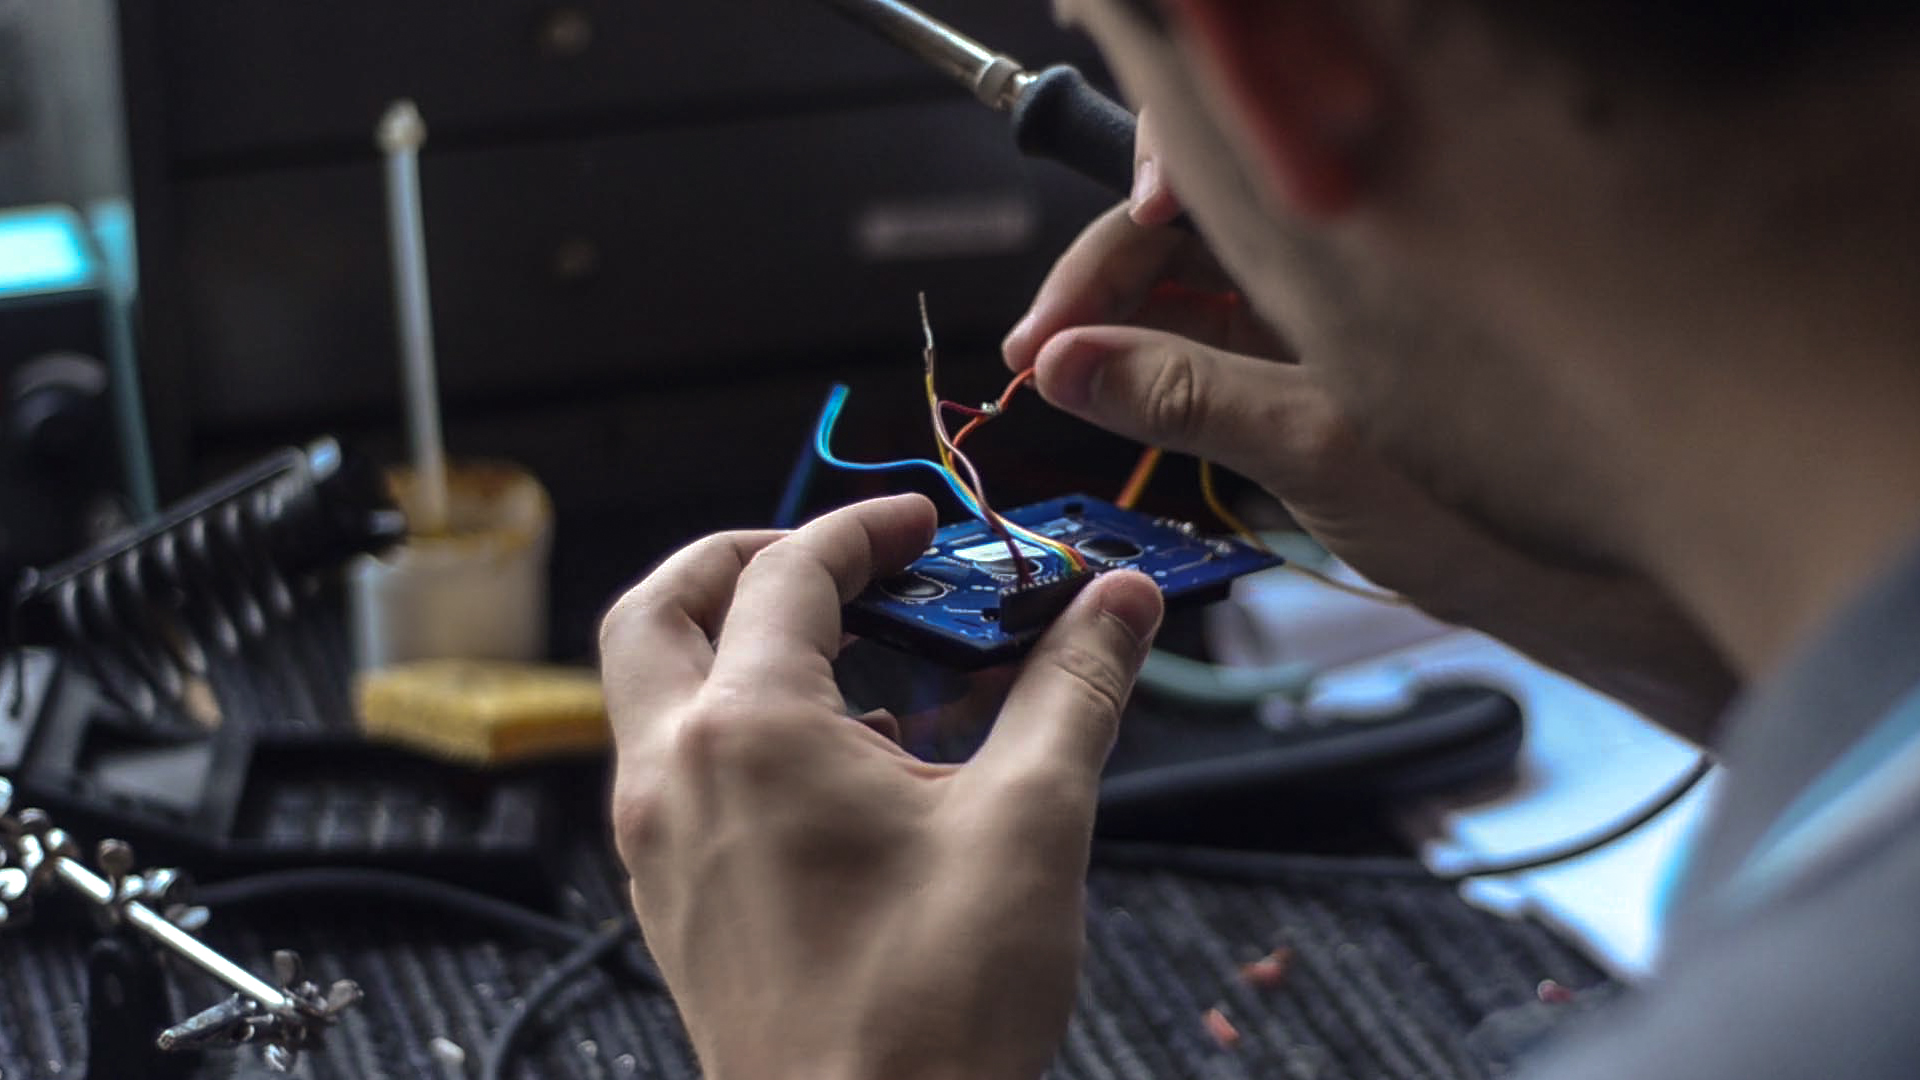
\includegraphics[width=\paperwidth]{soldering.jpg}

		\vspace{-12mm}

		\definecolor{light-gray}{gray}{0.85}
		\hfill {\scriptsize \color{light-gray} CC BY-NC-SA flickr.com/cbeas}
	\end{adjustwidth}

	\vfill

\end{titlepage}

\section{Der Verein}

Als erster Hackerspace\footnote{Mehr Informationen dazu gibt es auf
\url{http://hackerspaces.org/}} in Rapperswil-Jona bieten wir Computer- und
Technikbegeisterten seit August 2013 eine Plattform, in der sie ihr Wissen
weitergeben, austauschen und dazulernen können. Damit reihen wir uns in eine
weltweite Bewegung von tausenden von Vereinen ein.

Es geht dabei nicht um das ``Hacken von Computern'', wie es in den Medien häufig
dargestellt wird, sondern gemäss der ursprünglichen Definition eines
Hackers\footnote{Mehr zur ursprünglichen Definition eines Hackers gibt es auf
Wikipedia: \url{https://de.wikipedia.org/wiki/Hacker}} um den kreativen Umgang
mit Technik und Wissen. Wir bieten Infrastruktur und KnowHow, um
nichtkommerzielle Projekte alleine oder in Kollaboration zu realisieren.

Die zwei Ziele des Vereins gemäss Vereinsstatuten sind:

\begin{itemize}
		\item Bereitstellung der Infrastruktur zur Arbeit an nicht-kommerziellen
			technischen Projekten.
		\item Förderung des Informationsaustausches an regelmässigen Treffen,
			speziell im Bereich der Technologie.
\end{itemize}

In unserem Hackerspace möchten wir einerseits die Möglichkeiten und das Umfeld
zur Umsetzung von interessanten technischen oder künstlerischen Projekten
anbieten, andererseits auch den Austausch von Wissen fördern. Dies kann
regelmässige Treffen, öffentliche Kurzvorträge oder auch Bildungsangebote und
Workshops für interessierte Aussenstehende beinhalten.

\section{Projekte}

Damit Sie sich ein Bild unserer Aktivitäten machen können, nachfolgend drei
unserer aktuellen Projekte:

\textbf{Ferienpass im Computer- und Technikbereich}

Im November 2014 boten wir zum ersten Mal im Rahmen des Ferienpasses
Rapperswil-Jona\footnote{\url{Website: http://fepa-rj.ch/}} einen Löt- und einen
Programmierkurs für Kinder an. Diese -- wie auch wir selbst -- waren davon
begeistert: Wir erhielten 86 Anmeldungen und konnten davon aus Platzgründen
leider nur 16 berücksichtigen. Auch im Herbst 2015 boten wir die Kurse wieder
an, mit sehr positivem Feedback. Wir freuen uns, auch in Zukunft weiterhin
Schulkinder aus Rapperswil-Jona mit Technik in Kontakt zu bringen und dafür zu
begeistern.

\newpage
\textbf{Wassertemperatursensoren Zürichsee}

Aktuell ist es für badefreudige Personen am Obersee schwierig, herauszufinden
wie warm oder kalt der See aktuell ist. Wir möchten deshalb in Kooperation mit
lokalen Vereinen den Obersee (und später den Rest des Zürichsees) mit einem
Netzwerk aus solarbetriebenen Wassertemperatur-Sensoren ausstatten und diese
Messdaten öffentlich zugänglich machen.

\textbf{3D-Druck}

Letztes Jahr durften wir unseren ersten 3D-Drucker in Betrieb nehmen, finanziert
über die erfolgreiche Schweizer Crowdfunding-Plattform ``Wemakeit''. Im Rahmen
dieser Aktion haben wir unter anderem mit Hilfe eines Quadrokopters einen
3D-Scan des Schlosses Rapperswil erstellt, diese Daten in Kooperation mit der
Hochschule für Technik HSR sowie dem Rapperswiler Start-Up ``Drei-De''
aufbereitet und ein druckfertiges Modell erzeugt.

Dieses Jahr möchten wir gerne im Rahmen des Ferienpasses auch 3D-Druck-Workshops
durchführen.

\section{Weitere Informationen}

Weitere Informationen zu uns und unserem Verein finden Sie auf unserer
Website:\\\url{https://www.coredump.ch/}.

Für Rückfragen können Sie den Vorstand unter \url{vorstand@lists.coredump.ch}
kontaktieren.


% \section{Die Gründungsmitglieder}
% 
% Wir sind fünf technikbegeisterte Studenten oder Absolventen der
% Studienrichtungen Informatik oder Elektrotechnik an der Hochschule für Technik
% Rapperswil. Wir möchten den kreativen Umgang mit Technik fördern und
% interessierten Personen den praktischen Einstieg in die Elektronik und
% Informatik ermöglichen.
% 
% Als Studenten hätten wir natürlich auch im Rahmen der Hochschule einen solchen
% Verein gründen können, allerdings wäre dieser dann nur für Studenten zugänglich
% und würde Absolventen sowie nicht-studentische Interessenten ausschliessen.
% Deshalb haben wir uns bewusst dafür entschieden, einen von der HSR unabhängigen
% Verein zu gründen.

% \section{Mitglied werden?}
% 
% Egal wie viel Erfahrung du im Bereich der Informatik, Elektronik oder sonstwo
% hast, bei uns kann jeder Mitglied werden der sich für kreativen Umgang mit
% Technik interessiert und motiviert ist, Neues zu lernen.
% 
% Die Mitgliedschaft als Nichtverdiener kostet 10 CHF im Monat. Für Verdiener sind
% es 20 CHF.
% 
% Weitere Informationen findest du auf \url{https://www.coredump.ch/} oder per
% Email an \url{vorstand@coredump.ch}.

\end{document}
